%%%%%%%%%%%%%%%%%%%% author.tex %%%%%%%%%%%%%%%%%%%%%%%%%%%%%%%%%%%
%
% sample root file for your "contribution" to a contributed volume
%
% Use this file as a template for your own input.
%
%%%%%%%%%%%%%%%% Springer %%%%%%%%%%%%%%%%%%%%%%%%%%%%%%%%%%

% RECOMMENDED %%%%%%%%%%%%%%%%%%%%%%%%%%%%%%%%%%%%%%%%%%%%%%%%%%%
\documentclass[graybox]{svmult}
% choose options for [] as required from the list
% in the Reference Guide
\usepackage{mathptmx}       % selects Times Roman as basic font
\usepackage{helvet}         % selects Helvetica as sans-serif font
\usepackage{courier}        % selects Courier as typewriter font
\usepackage{type1cm}        % activate if the above 3 fonts are
                            % not available on your system
%
\usepackage{makeidx}         % allows index generation
\usepackage{graphicx}        % standard LaTeX graphics tool
                             % when including figure files
\usepackage{multicol}        % used for the two-column index
\usepackage[bottom]{footmisc}% places footnotes at page bottom
%\PassOptionsToPackage{hyphens}{url}
%\usepackage{fullpage}
\usepackage{url}
\usepackage{hyperref}
\usepackage{doi}
%\usepackage{natbib}
\usepackage{amssymb}
\usepackage{epstopdf}
\usepackage{wrapfig}
%\DeclareGraphicsRule{.tif}{png}{.png}{`convert #1 `dirname #1`/`basename #1 .tif`.png}
% see the list of further useful packages
% in the Reference Guide

\makeindex             % used for the subject index
                       % please use the style svind.ist with
                       % your makeindex program
\newcommand{\putabstract}{ Musical performances with touch-screen
  devices can be recorded by capturing a log of touch interactions.
  This new-media object can serve as an archive or as a basis for
  other representations of the musical work. This paper presents a
  protocol for logging touch-interactions as well as visualisations
  and gesture-scores generated from logs of a series of improvised
  ensemble performances on iPads. These objects record the
  performances for posterity and also allow deeper analysis of musical
  interactions present. }
%%%%%%%%%%%%%%%%%%%%%%%%%%%%%%%%%%%%%%%%%%%%%%%%%%%%%%%%%%%%%%%%%%%%%%%%%%%%%%%%%%%%%%%%%

\begin{document}

\title*{A Percussion-Focussed Approach to Preserving Musical
  Performance on Touch-Screens (draft)}
% Use \titlerunning{Short Title} for an abbreviated version of
% your contribution title if the original one is too long
\author{Charles Martin and Henry Gardner}
% Use \authorrunning{Short Title} for an abbreviated version of
% your contribution title if the original one is too long
\institute{Charles Martin \at Research School of Computer Science, The
  Australian National University, Canberra,
  \email{charles.martin@anu.edu.au} \and 
  Henry Gardner \at
  Research School of Computer Science, The Australian National
  University, Canberra, \email{henry.gardner@anu.edu.au}}

\maketitle
\abstract*{\putabstract}
\abstract{\putabstract}

\section{Introduction}

As an artistic experience, musical performance is fleetingly temporal
and the history of music abounds with technologies and traditions to
grab hold of musical performances, recording them in some format to be
archived, understood, and developed. All of our traditions of musical
recording, from rote-learning and notation, to the phonograph and
digital recording, have contributed to the ability of performers to
create new musical works and to the place of music in our cultural
landscape.

While western classial music is often defined by the score, and
popular music by the song or the recorded version, the practice of
free improvisation often defies the identification of a canonical
``musical work''. In free-improvised ensemble music, all decisions
about the notes to play are made in the moment by individual musicians
with the work ending only when all performers have stopped playing.
With each performance equally identifiable as a different work, the
output of free-improvisation ensembles is often represented only as
audio recordings with documented changes in personnel or
instrumentation the main indicator of difference between works. When
performing with computer-based instruments, however, musicians have
the opportunity to record the musical work in an extremely detailed
form by capturing a log of their interactions as well as audio or
video recordings.

In this chapter, we present a protocol for automatically documenting
free-improvised musical performances made on touch-screen computers.
Our protocol, and the touch-screen instruments with which it is used,
are designed from a percussionist-centred perspective. Rather than
particular notes and rhythms, the focus of traditional musical
notation, our protocol records detailed touch movements in absolute
time and abstract touch gestures identified during the performance by our
computer software. Given that ensemble interactions are one of the
most interesting aspects of free-improvised music, our protocol is designed
to connect to multiple touch-screen devices engaged in ensemble
performance over a local network or the internet.

We argue that this protocol can serve as an archival format that
addresses many of the issues with curating improvised music for the
specific case of performances on touch-screens. Not only does it allow
a much more comprehensive documentation of the performances, but it
allows these performances to be characterised, analyised, and
appraised through statistics calculated on the touch and gestural data
which is abstracted from the particular instruments used or the
musicians who played them. We also show how logs of touch-screen
performances can become new media art objects in their own right,
forming a basis for other representations of the improvised musical
work such as visualisations or scores.

We will describe our protocol for capturing touch interactions and how
it has developed from previous schemes for capturing and controlling
musical performances. We will also present the statistics and
visualisation tools used for analysing and comparing performances
documented with our protocol. Our protocol and these tools were
developed as part of a series of research projects in touch-screen
musical performance and we will discuss how they have influenced the
research and artistic outcomes of these projects. In particular, we
will discuss the experiences of using these systems with Ensemble
Metatone, a free-improvisation percussion group that participated in a
longitudinal study over eighteen months performing with our
touch-screen instruments.

% Although this protocol was developed for research purposes,
% visualisations and analyses generated from logged data has formed an
% important archive of the group's performances of \emph{MetaLonsdale}
% for four iPads

% motivations: mode of interacting with multiple iPad performers
% deep documentation
% new forms of analysis

\footnote{\label{note1}The video recording, touch-interaction log,
  visualisation and score of a performance of \emph{MetaLonsdale} is
  available online:
  \url{http://charlesmartin.com.au/blog/2014/1/17/metalonsdale-for-four-ipads}.}

\section{Percussive Improvisation on touch-screens}

% stuff about how percussion has an approach to music and
% improvisation defined by gesture and how this makes it an
% appropriate praxis for viewing touch-screen performance

The development of our touch-screen instruments and performance
logging protocol was a percussionist-centred process. Performances and
rehearsals, of Ensemble Metatone a free-improvising percussion
ensemble were conducted to explore and evaluate instruments and our
performance logging protocol was developed to document and analyse
these activities. Before detailing the protocol and instruments it is
worth considering why percussive improvisation is a useful process not
just for exploring musical interaction but for characterising it.

\subsection{Percussive Interaction}

Percussion is an artistic practice defined by an approach to
interaction rather than by any particular instrument that
percussionists play. Percussionists perform by ``striking, scraping,
brushing, rubbing, whacking, or crashing any... available
object''~\cite{Schick:2006fk}. Blades~\cite{Blades:1992kx} discusses
the earliest percussion instruments, idiophones, where the body of an
instrument creates the sound, rather than an air column or string. He
divides them by their method of interaction: ``shaken'', ``stamping''
(played with the hands or feet), ``scraped'', ``concussion'' (two
parts struck together), and ``struck'' (with a stick or non-sounding
implement). These descriptions match taxonomies of modern instruments
(such as Cook~\cite{Cook:1997vn}) and focus on the mode of interaction
for the instruments rather than their physical design.

Modern percussionists are accustomed to exploring non-traditional
objects to create music and use these percussive gestures to coax wide
varieties of timbres and musical gestures from simple instruments.
Performers of Xenakis' \emph{Psappha}~\cite{Xenakis:1975uq} or
Feldman's \emph{King of Denmark}~\cite{Feldman:1965uq} must design
their own multi-instrument setup to fit the composer's specifications.
To meet the requirement for metal instruments, for example, a
performer might find a car's suspension spring, a saw-blade or create
a unique object from scratch.

For percussionists, free improvisation is often a process of gestural
exploration, discovering new sounds from traditional and
non-traditional instruments and responding to other sounds in an
ensemble. Like some of the instruments in a modern percussion
ensemble, touch-screen computing devices can be struck, scraped and
rubbed with fingers and hands. Their percussive affordances, their
power to generate computer music and their widespread popularity,
motivate an exploration of the use of touch-screen devices in a modern
percussion ensemble.

\subsection{Composing with Gestures}

While traditional musical notation specifies sonic outcomes - pitch,
articulation and rhythm - it is possible to compose music by
specifying gestures used for interacting with instruments. For
percussionists, where gestures are transported across a variety of
instruments, this is a popular way of notating music for particularly
unconventional instruments. Thierry de May's famous work \emph{Music
de Tables}~\cite{May:1987fk} is written for three percussionists who
perform on the surfaces of regular tables. de May defines a vocabulary
of notation for gestures that are used with standard rhythmic notation
in the score. Burtner's \emph{Syntax of Snow}~\cite{Burtner:2011fk}
asks the solo performer to play a glockenspiel with one hand and a
bowl of snow with the other. The score sets out a complex scheme of
gestures for ``playing'' the snow, with a pair of symbols (see Figure
\ref{fig:SyntaxOfSnow}) for each gesture, representing the type of
gesture as well as hand position in the bowl.

\begin{table}\centering
\begin{tabular}{|l|}
\hline
touch lightly \\
fingers tapping \\
sift through fingers \\
with closed fist\\
crush in hand\\
pat with open palm\\
drop handful\\
flick with fingernail\\
draw line\\
resonant thump\\
press on surface\\
swish with palm\\
\hline
\end{tabular}
\label{tab:SyntaxOfSnowGestures}
\caption{The vocabulary of gestures to perform on the amplified snow
  in Burtner's \emph{Syntax of Snow}. Each gesture is represented by a
  symbol in the score and are played simultaneously with notes on the glockenspiel.}
\end{table}


\begin{figure}[h] \centering
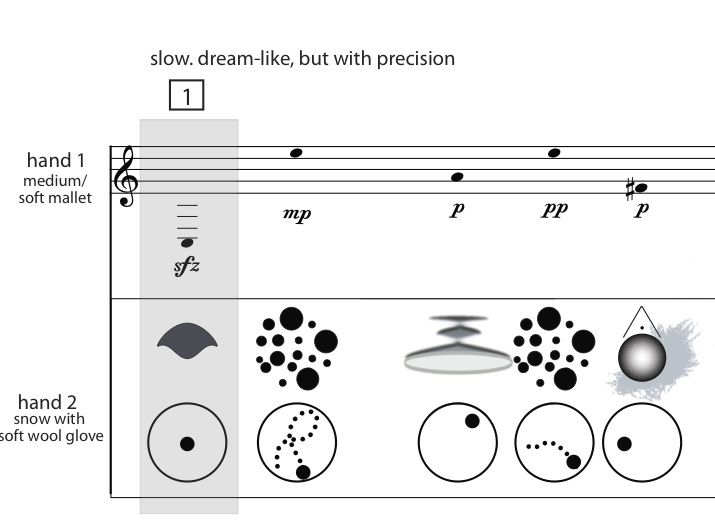
\includegraphics[width=0.7\columnwidth]{figures/syntaxofsnow-excerpt.jpg}
\caption{An excerpt from Matthew Burtner's \emph{Syntax of
    Snow}~\cite{Burtner:2011fk} for solo glockenspiel and bowl of
  amplified snow. The composer defines a vocabulary of
  gestures for interacting with the snow with one hand represented by
  symbols below a regular staff for notes on the glockenspiel.}
\label{fig:SyntaxOfSnow}
\end{figure}

Although Burtner's vocabulary of gestures is specific to the
particular case of performing with snow, some of the gestures (e.g
``touch with finger'', ``swish'', ``draw line'') could generalise to
other instruments and to touch-screens. For documenting performances
on touch-screens it will be necessary to characterise a vocabulary of
gestures that is common to many different types of instruments that
can be implemented on touch-screen devices and can express a wide
variety of playing styles.

It is notable that many of the gestures indicated in Burtner's score
could be interpreted as being continuous rather than ceasing after a
following the instruction. For example, ``fingers tapping'' should
probably be interpreted not as one or two taps but as a continual
tapping until the performer reaches the next instruction. In HCI
research, gestures on touch-screens are frequently characterised as a
having a short and finite expression, as they are usually designed to
execute a command in software (e.g. double tap to open a menu) rather
than to create an artistic expression. For this reason,
characterisations of touch gestures that already exist in the HCI
literature are unsuitable for characterising performative touch
gestures which, as we will demonstrate, mainly consist of continuous
interactions. 

\subsection{Free-Improvised Performance}

Free improvised performance has been defined as the performance of
music ``without any restrictions regarding style or genre and without
having predetermined what is to be played''~\cite{Stenstrom:2009xy}.
This definition is a typical of the field, but it frames
free-improvisation subtractively: improvisation is ``regular''
performance minus restrictions. To understand what is really exciting
about free-improvisation as mode of artistic expression and as a
methodology for researching unfamiliar interactions, we must look at
what free-improvisation \emph{adds} to performance. Bill Cahn, member
of the pioneering percussion group, Nexus, writes that improvisation
encourages ``a deeper knowledge of the instruments and their
sound-making possibilities''~\cite{Cahn:2005uq}. Digital media
theorist Aden Evens writes that when improvising with an unfamiliar
instrument ``the musician generates novel and surprising results even
when applying familiar technique.''~\cite{Evens:2005kx}

Although it is rare for free-improvisations to be subjected to an
internal musical analysis, unlike other forms of music including jazz
improvisations, some characterisations of the internal structure of
these performances have been published.
Pressing~\cite{Pressing:1988uo} has developed a model of improvisation
that divides performances into a series of non-overlapping events
separated by trigger points during the performance that initiate each
event. Stenstr\"om proposes a terminology for free ensemble
improvisation, including concepts such as ``transitions'' between
musical ideas and ``attractors'' such as a steady pulse that encourage
similar playing from other performers~\cite{Stenstrom:2009xy}.
Nunn~\cite{Nunn:1998ly} similarly argues that a ``segmented form''
divided by ``transitions'' is the fundamental structure of free
improvisation.

\subsection{Ensemble Metatone and improvising iPad ensembles}

In the present research, an improvising percussion group was not only
the used to create new music but to explore and evaluate touch-screen
instruments running on Apple iPads. Ensemble Metatone was brought
together in Canberra, Australia to study the process performing
free-improvised music starting with a prototype app and, through a
process of iterative design, eventually presenting concerts with
multiple apps. The members of the group (including one of the authors)
were all trained in classical percussion and had significant
experience as improvisors.

Ensemble Metatone undertook a series of studio rehearsals throughout
2013 to develop a repertoire of free-improvised music with our iPad
apps~\cite{Martin:2014jk}. Using a process of ``creative music
making''~\cite{Cahn:2005uq} where improvisations are followed by
critical listening and discussion, the performers developed a
vocabulary of touch interactions inspired by their percussion
training. Notably, they also discovered novel sounds from the
instruments that could be created with unusual or atypical
interactions and were not foreseen by the app
designer~\cite{Martin:2014cr}. The performers of Ensemble Metatone
settled on a combination of iPad and acoustic percussion instruments
allowing them to choose from a wide palette of sound colours in their
performances. The initial series of rehearsals was followed by a
recorded research concert with a live audience, a series of
performances at experimental art events. The recording of Metatone's
research concert was released as a digital album in March
2014~\cite{Ensemble-Metatone:2014sf}.

Other percussion performers were also invited to work with our
touch-screen apps in a variety of improvised and semi-composed
performances in Australia and the USA. In 2014, a number of Metatone
apps were made available for free in the Apple iTunes App Store and
the authors are aware of several performances using the apps unrelated
to our work.

In 2015, the Metatone apps were used as part of the educational
activities of the New Music Ensemble at the ANU School of Music
including rehearsals and performances and in activities with
high-school students. In this setting participants had a range of
instrumental experience so iPads were used as the only instrument. A
formal study was conducted with four iPad quartets, including members
of the New Music Ensemble and volunteers from the local music
community, who performed several improvisations with different
combinations of software features.

The majority of these rehearsals and performances were audio and video
recorded and also documented using our touch-screen performance
protocol. To date, we have archived over 80 performances of our iPad
apps using these tools forming a highly comprehensive corpus of work
for studying improvisation on touch screens. In the following
sections, we will describe forms of analysis and derivative works that
can be generated from this archive of performance documentation.

% Over a series of studio rehearsals, the group worked with the
% ``MetaLonsdale'' app to develop a work which was performed at
% festivals and events throughout 2013. The studio rehearsals and a
% public recital were recorded with seperate tracks of audio for each
% iPad, multiple camera angles, and a log of touch-interactions.

% The app used a percussion-inspired interaction scheme allowing
% performers to access pitched percussion sounds and field recordings.
% Most of the iPad screen was a performance surface with few graphical
% UI elements. Tapping the screen produced short sounds at a pitch
% determined by the location of the tap. Swiping played continuous field
% recordings with volume controlled by the velocity of the swipe. The
% app featured two UI switches that controlled simple delay functions,
% that repeat tapped notes, and switchable auto-play features, that
% alogrithmically produced background sounds. A button on both apps
% allowed the performer to shuffle the available sounds.

\begin{figure}
  \centering
  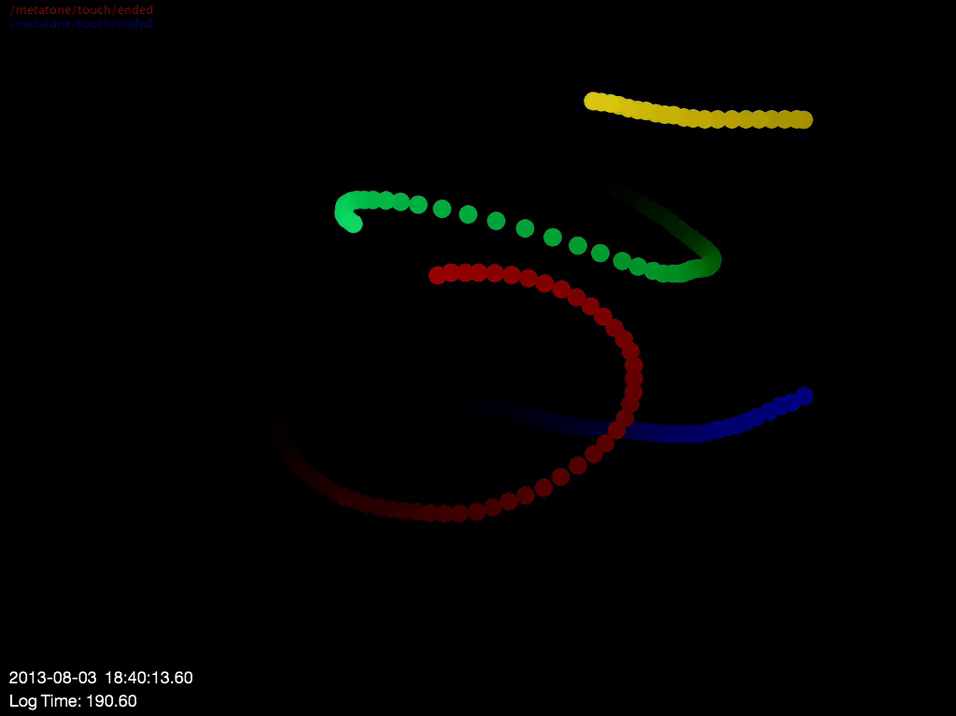
\includegraphics[width=0.5\textwidth]{figures/metatoneanimation1}
  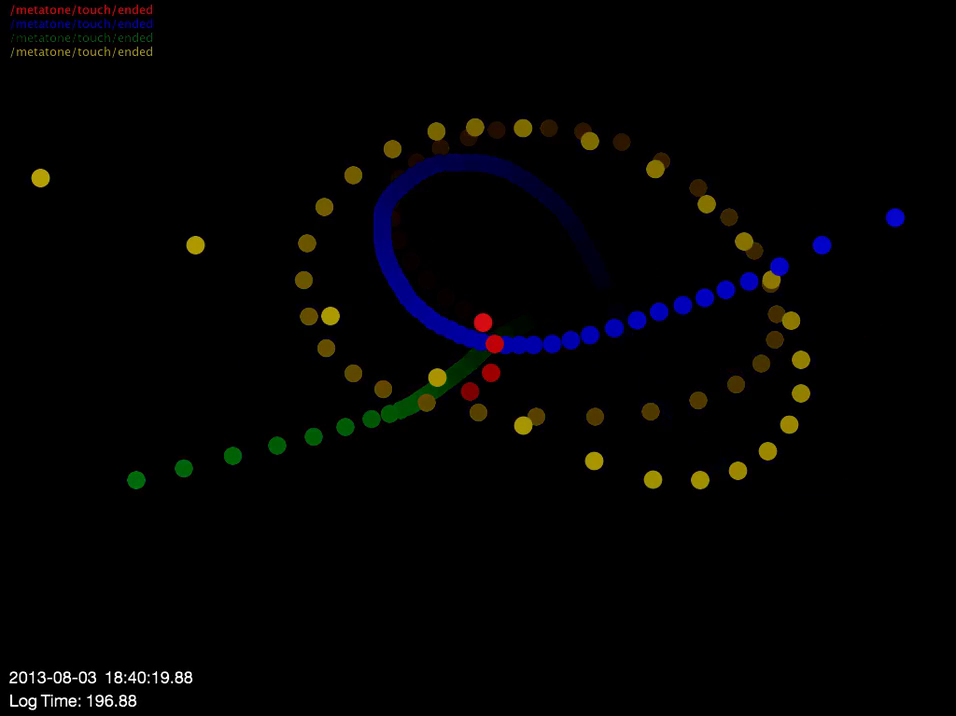
\includegraphics[width=0.5\textwidth]{figures/metatoneanimation3}
  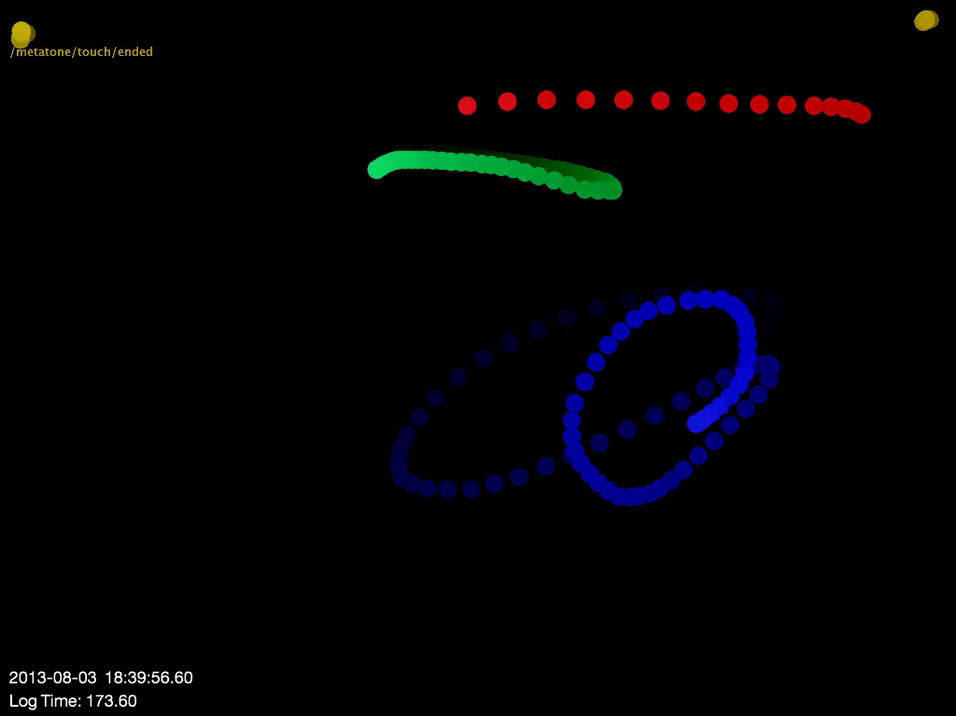
\includegraphics[width=0.5\textwidth]{figures/metatoneanimation2}
   \caption{Stills from an animation of an Ensemble Metatone
     performance. The full animation can be viewed online\footref{note1}.}
  \label{metatoneanimation3}
\end{figure}

\section{Curating the Improvised}

Although the field of improvised performance has a developing
theoretical background and many highly regarded practitioners,
particular artistic expressions tend toward the ephemeral. In the
following sections, we describe our approach to recording improvised
performances on touch screen and transforming such transcriptions into
animations and gestural sequences. These can be generated after
performances for the purposes of archiving and research as well
as produced in real-time as additional aspects of the live improvised work.

\subsection{Representing the Musical Work}

\begin{figure}
  \centering
  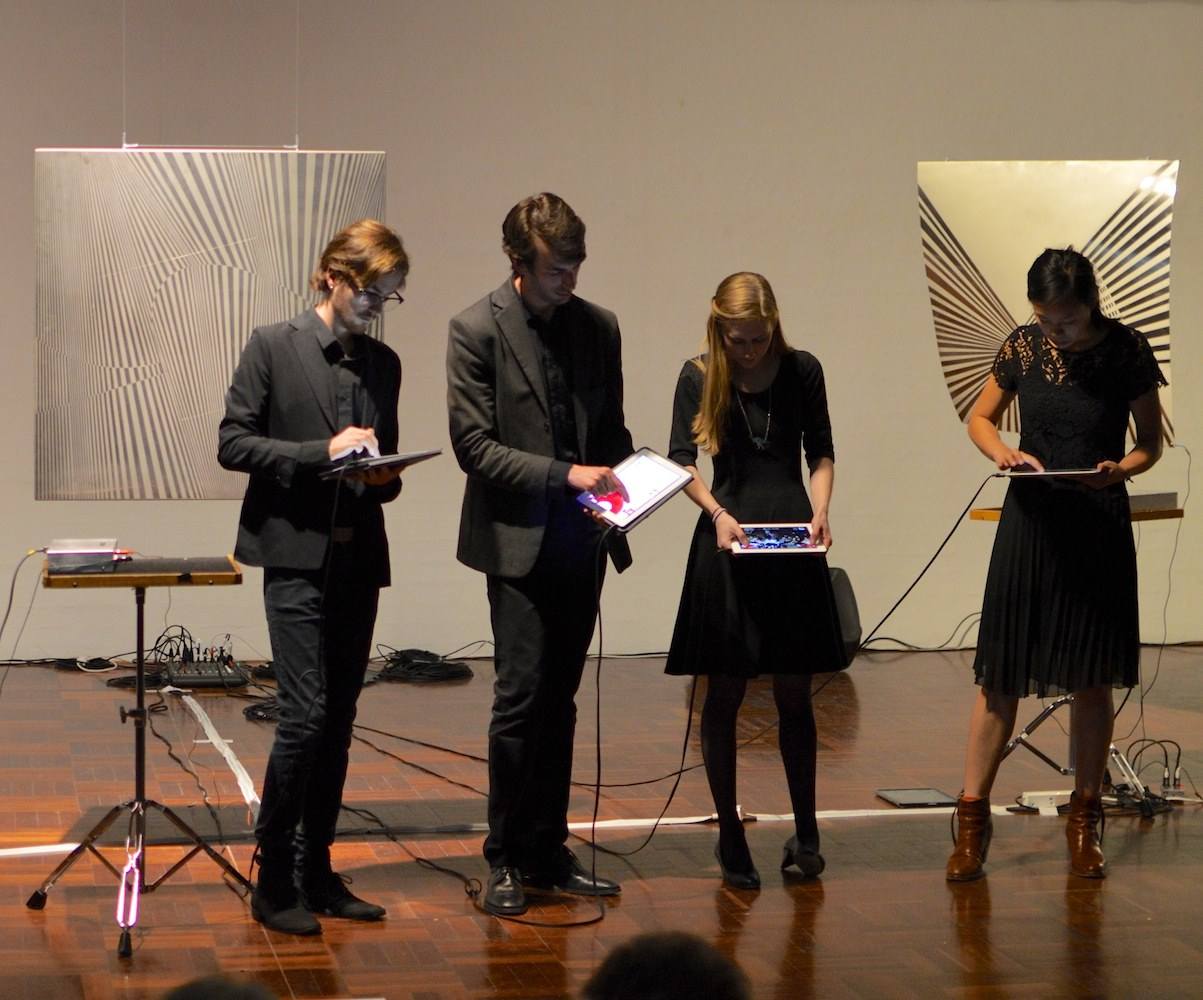
\includegraphics[width=\textwidth]{figures/ensemblemetatone}
  \caption{Ensemble Metatone performing \emph{MetaLonsdale} at the ANU
    School of Art Gallery in October 2013 (left to right: Jonathan
    Griffiths, Charles Martin, Christina Hopgood, Yvonne Lam).}
  \label{ensemblemetatoneperforming}
\end{figure}

It is widely recognised that musical works as well as new media
artefacts can have a number of interacting
representations~\cite{Rinehart:2007pi}. Musical works might be
directed by a score; be ``thick'' or ``thin'' depending on the the
freedom of interpretation afforded the performers; be represented in
live performance, studio recordings, or by computer generated
renderings; and may be composed or improvised~\cite{Davies:2005fj}.
Combinations of these representations are often collected together
form an archive of a musical work.

Free improvised music, where performers do not follow a set musical
structure, is usually preserved using only audio and video recordings.
While the improvised solos of famous jazz musicians are often
transcribed, this is extremely uncommon for free-improvised ensemble
performances. For improvised music on touch-screens, a log of
touch-interactions captured by the performance suplements traditional
recordings and could take the place of a ``score'' in documenting such
performances. While scores are generally used for composition, their
use as documentation for new media artworks has been
acknowledged~\cite{MacDonald:2009ve}. Such a log would also satisfy
Manovich's principles for a new media artwork~\cite{Manovich:2002ly}.
In particular, the log of touch-interactions is variable, forming the
basis for derivative artworks that also represent aspects of the
original performance.

Free-improvisation is often a process of gestural exploration,
discovering new sounds and responding to other sounds in an ensemble.
In audio recordings of these performances, the sonic result of the
gesture is captured but the gesture itself lost. While the gestural
component of musical performance may not be as integral as in dance or
other physical performance, it still contributes to the audience's
perception of a work and represents a certain amount of the
performers' intention. Although touch-interaction data is not a
complete record of performers' gestures it is simple to obtain and
easily transformed into other representations of a performance.

% - percussion interaction - more details
% - composing with gestures - more details (e.g. from TPR 2013.
% - comparison to TUIO: \cite{TUIO_KBBC05}


\section{Protocols for musical touch interaction}
\label{sec:protocols}

In performances with our iPad apps, all touch interactions during the
performance are transmitted over a Wi-Fi network to server software
running on a laptop or a remote virtual server. We have developed a
relatively simple protocol for formatting touch and other interaction
data using the OSC~\cite{osc-nime2009} (Open Sound Control) standard.
The data is transmitted either through Unix sockets using the UDP
protocol (as is typical for OSC messages) or through
WebSockets~\cite{Fette:2011eu}, which is the preferred method due to
increased reliability of transmission and the ability to easily open a
bi-directional connection with a remote server. 

\subsection{Protocols for capturing performance data}
\label{subsec:protocols}

Musical data has been abstracted from the temporality of performance
for centuries since the development of musical notation. Mechanical
instruments such as music boxes and barrel organs developed in the
18th century~\cite{Fowler:1967kq} first allowed music to be
``programmed'' rather than performed. More refined mechanical
instruments such as the ``reproducing piano'', which appeared at the
turn of the 20th century~\cite{Kapur:2005fk}, allowed a musician's performance to be
automatically transcribed and converted into a paper ``piano roll''
that could be re-played many times. All of these technologies have had
an impact in the study of music as well as it's performance. Musical
notation enabled the field of musicology, where the musical score has
traditionally been priveleged as the canonical representation of a
musical work. The piano-roll performances of many famous pianists were
made before audio recording was available or widespread and have been
used to analyse their performance styles.

An important antecedent of our work was the
MIDI~\cite{midi1996complete} (Musical Instrument Digital Interface)
protocol, which was developed in the late 1970s to connect electronic
music \emph{controllers}, such electronic versions of keyboards, drums
and wind instruments and new musical interfaces such as ``THE
HANDS''~\cite{TheHandsArticle}, with electronic synthesisers or
digital recording systems. While this standard was intended as a
control interface for live performance or recording, it was subverted
by digital artists and researchers who recognised that the MIDI trace
of a musical performance could be used for other purposes. MIDI was
originally designed to be used with a physical serial connection
however virtual MIDI connections are commonly used to connect multiple
pieces of software on one computer system and a networked version of
MIDI also exists\cite{Lazzaro:2004pb}.

While the success of MIDI is ongoing, the semantics of the protocol is
mostly restricted to a keyboard and note perspective on musical data.
The typical MIDI interactions are ``note on'' and ``note off''
messages, each of which contain a pitch and dynamic (volume) value.
Changing parameters while a note is playing can be achieved by
simultaneously sending one of a limited number of ``continuous
control'' messages while the ``note on'' is held. In an effort to
develop a semantics-free format for musical control that better
reflected the needs of modern computer music systems,
OSC~\cite{osc-nime2009} (Open Sound Control) was developed which
defines a standard message format but with the specific content of the
messages up to the application developer. This flexibility has
contributed to the success of OSC not just in computer music, but in
professional applications such as show control~\cite{schmeder2010best}
although it is not commonly available in commercial electronic
instruments.

Some have attempted to define protocols using OSC to standardise
interaction with certain types of interface. TUIO~\cite{TUIO_KBBC05}
is one such protocol designed for table-top interfaces where special
objects, ``fiducial markers'', could be tracked as well as finger
touches. Unlike MIDI, TUIO does not define the purpose of messages but
communicates only information about basic components that the
designers expected would be common to most table-top interfaces. The
TUIO protocol sends groups of messages together that encompass the
state of the whole table-top interface. Most importantly, one
\texttt{set} message is sent for each object on the surface that has
changed position. A \texttt{set} message includes
identification and position information about the object being tracked
as well as precalculated data such as velocity, acceleration, and
rotation. This simplifies the requirements for software receiving TUIO
which may not have to keep track of objects in between bundles of of
messages or worry about errors due to messages arriving out of order.

\subsection{Touch Screen Data}
\label{subsec:touch-screen-data}

Like TUIO our protocol for logging touch-screen performances needed to
capture the fundamental interactions occuring on the touch-screen, not
how these interactions are interpreted by the application currently
running on the device. In Apple iOS devices, data collected from the
multitouch digitiser in front of the screen is interpreted by the
operating system which keeps track of individual touches and divides
the incoming data into events~\cite{AppleDeveloper:2015rm}. Software
developers can implement a set of callback functions to access these
events individually. So-called \texttt{UIEvent}s track the state of
touches on the screen - they ``begin'', ``move'', ``end'', and may be
``cancelled'' if they are mis-recognised. For the purposes of
designing software for free-form touch improvisation, only the first
three states are of interest. The touch-data objects described by
these events have a record of their current as well as previous
location on the screen. A value proportional to instantaneous velocity
of moving touches can be easily calculated by finding the length of
the vector from the previous location to the new.

\begin{figure}
\begin{verbatim}
- (void)touchesBegan:(NSSet *)touches 
    withEvent:(UIEvent *)event;
- (void)touchesMoved:(NSSet *)touches 
    withEvent:(UIEvent *)event;
- (void)touchesEnded:(NSSet *)touches 
    withEvent:(UIEvent *)event;
- (void)touchesCancelled:(NSSet *)touches 
    withEvent:(UIEvent *)event;
\end{verbatim}
\caption{Callback methods for accessing touch events in
  Apple iOS~\cite{AppleDeveloper:2015rm}. Our Metatone apps log each
  \texttt{touchesBegan}, \texttt{touchesMoved}, and \texttt{touchesEnded} event.}
\label{touch-event-code-listing}
\end{figure}

\subsection{Metatone Apps}
\label{subsec:metatone-apps}

The touch-screen device chosen for our research and performances was
the Apple iPad. A variety of apps have been developed so far for
performances with Ensemble Metatone and other groups. All the Metatone
apps share the same fundamental mode of interaction: a tap triggers a
single sound with a percussive envelope (i.e. a sharp attack and long
decay), while swiping plays a continuous sound with volume related to
the velocity of the moving touch. Apart from this commonality, the
Metatone apps feature different palettes of available sounds and modes
of synthesis, different arrangements of sounds on screen, a variety of
special features, and different kinds of networked interactions between
the iPads themselves as well as with a server application.

\subsection{The Metatone Log Format}
\label{subsec:metatone-log}

During performances with our iPad apps, all touch interactions are
transmitted as OSC messages over a Wi-Fi network from the iPads to
server software running on a laptop, or on a remote server. When our
server receives one of these OSC messages, it assigns it a timestampe
and records it to a text file for later analysis. Each line of the
text file is written in the CSV (comma separated values) format.
Although the different aspects of the performance are recorded using
different numbers of parameters, these can be trivially separated or
reorganised by filtering through the unique OSC address of each type
of message. 

Messages are sent in response to three of the four touch-events in
iOS, \texttt{touchesBegan}, \texttt{touchesMoved}, and
\texttt{touchesEnded}. Both \texttt{touchesBegan} and
\texttt{touchesMoved} are recorded using a \texttt{/metatone/touch}
message recording the iPad's app-level unique device ID. The velocity
of \texttt{touchesMoved} messages is recorded while
\texttt{touchesBegan} messages are distinguished by having a velocity
of zero. A \texttt{/metatone/touch/ended} message is used to record
\texttt{touchesEnded} events. \texttt{touchesCancelled} messages are
ignored.
 
Each of our iPad apps contains a small number of button and switch UI
elements that are used in the performances to activate looping
functions, algorithmically generated backing sounds, and to change the
timbre and pitch of sounds available through the touch interface. The
performers' interactions with these elements are recorded using
\texttt{/metatone/switch} messages which record the iPad device ID,
the name of the UI element and its new state.

During performances, our iPad apps send messages to the other apps
performing while connected on the same local network. These messages
are also copied to the server software using the
\texttt{/metatone/app} OSC address.

As will be described in later sections, our server software has the
capacity to identify the performers' touch gestures in real-time
during performances. The server tracks these gestures to identify the
whole state of the whole ensemble and, in particular, identify moments
of peak gestural change where the group may have moved onto a new
musical section. While this information is recorded for later
analysis, it is also returned to the performers' apps, which use it to
update their interfaces and present new performance possibilities to
the performers~\cite{Martin:2015jk}. Our protocol for performance logging includes three
OSC messages from the server to the iPad apps. Gesture classifications
are returned to the iPads each second using the OSC address
\texttt{/metatone/classifier/gesture}; whenever a new musical section
is detected, the server sends a
\texttt{/metatone/classifier/ensemble/event/new\_idea} message to all
connected iPads; finally, various measures of the ensemble state are
returned to the iPads each second using the OSC address,
\texttt{/metatone/classifier/ensemble/state}, although this
functionality is still in development.

This scheme for logging touch-interactions (see table \ref{oscschema})
was chosen to study the process of improvising with iPad instruments
and not necessarily for replaying performances. Other aspects of the
touch-screen state such as unique identifiers for each touch point are
not tracked, nor are the exact pitches available on screen for each
player. Multitracked audio recordings of performance are deemed to be
sufficient record of the particular sounds created during the
performance while the touch protocols store the details of performers'
interaction with the instruments that the audio recording cannot.
While our protocols were created for research purposes, the CSV
storage format allows us to easily transform these logs into
alternative representations of performances.
The next section will describe these new outputs, and how they not
only aid in understanding the improvised performances, but serve as
representative artefacts along with audio and video recordings.

\begin{table}
  \begin{center}
  App to Server Messages:\\

  \begin{tabular}{|l|l|}
  \hline
  OSC Address           & Parameters \\ 
  \hline
  \texttt{/metatone/online}      & device  \\     
  \texttt{/metatone/touch}       & device, X, Y, velocity \\
  \texttt{/metatone/touch/ended} & device \\  
  \texttt{/metatone/switch}      & device, switch name, position\\
  \texttt{/metatone/app}         & device, message name, message state\\
  \hline
  \end{tabular}\\
  Server to App Messages:\\
  \begin{tabular}{|l|l|}
  \hline
  OSC Address           & Parameters \\ \hline
  \texttt{/metatone/classifier/gesture} & device, gesture type\\
  \texttt{/metatone/classifier/ensemble/event/new\_idea} & device, measure value\\
  \texttt{/metatone/classifier/ensemble/state} & type, value 1, value 2 \\
  \hline
  \end{tabular}
\end{center}
  \caption{Scheme for OSC messages from the Metatone iPad apps. The
    touch and touch ended messages record touch screen interactions
    directly from the iOS operating system (see Figure /ref{touch-event-code-listing}. The
    switch message was used to record interactions with UI elements
    (switches and buttons) present in our app where the name of the
    element is given as a string in the message.}
  \label{oscschema} 
\end{table}

\section{Analysing and Transforming Performance Logs}
\label{sec:analysis}

Our system of iPad apps and server software records all touch events,
UI interactions, and app-to-app communications that occur during
improvised performances with our iPad apps and records them in CSV
format. Our server software analyses these gestures during the
performance to produce more information about the performers'
interactions with the touch-screen devices and the state of the whole
ensemble. After performances, the touch protocols can be transformed
into gestural ``scores'' of the improvised pieces and into animations
of the performers' touch interactions. These representations of the
performance form a detailed archive of our improvised musical practice
and aid our efforts to analyse and understand touch-screen performance.

\subsection{Gesture Classification and Gestural Scores}
\label{subsec:gesture-classification}

Each second during performances, our server software analyses the
previous five seconds of touch-data from each connected iPad and
identifies the performers' current touch gesture. Our system
calculates feature vectors of descriptive statistics for each player
from these five-second windows of recorded touch interactions. The
feature vectors are classified using a Random Forest
Classifier~\cite{Breiman:2001kx} from the Python \texttt{scikit-learn}
library that is trained with examples of nine touch gestures recorded
by our app designer using a formal data collection
procedure~\cite{Martin:2015jk}. 

\begin{table}
\begin{center}
    \begin{tabular}{|l|l|l|l|}
    \hline
    \# & Code & Description & Group \\ \hline
    0 & N   & Nothing & 0 \\
    1 & FT  & Fast Tapping & 1\\
    2 & ST  & Slow Tapping & 1\\
    3 & FS  & Fast Swiping & 2\\
    4 & FSA & Accelerating Fast Swiping & 2\\
    5 & VSS & Very Slow Swirling & 3\\
    6 & BS  & Big Swirling & 3\\
    7 & SS  & Small Swirling & 3\\
    8 & C   & Combination of Swirls and Taps & 4\\ \hline
    \end{tabular}
\end{center}
\caption{The nine gesture classes that our server software, Metatone
  Classifier, can identify in touch screen performances. This
  vocabulary resembles the gestural language created for works such as
  Syntax of Snow (see Table \ref{tab:SyntaxOfSnowGestures}).}
\label{tab:gesture-classes}
\end{table}


The nine gesture classes are based on those discovered through
qualitative analysis of Ensemble Metatone's earliest series of
rehearsals~\cite{Martin:2014jk}. The vocabulary focusses on three
fundamental touch gesture groups: tapping, swiping, and swirling, and
it includes several variations of each group. Unlike other systems for
gesture recognition (cite) which are designed to interpret sequences
of movements with a beginning and ending as a command in a computing
interface\footnote{This includes Apple's built in
  \texttt{UIGestureRecognizer} class.}, our classification system aims
to segment a continuous stream of free form gestures. For this reason,
our vocabulary seeks to identify ``tapping'', which could continue
indefinitely, rather than ``tap'' which is completed after one touch
interaction. In this way, our touch-screen gestural vocabulary
resembles some of the snow gestures of \emph{Syntax of
  Snow}~\cite{Burtner:2011fk} which also are open ended which respect
to the number or length of interactions. 

Applying this gestural classification scheme to touch-screen
performances results in a new representation of the performance, that
is, a time-series of gesture classes at 1 second intervals for each
performer in the ensemble. Although this time-series does not contain
the details of each performer's interactions, it can still serve as a
kind of musical score for performances, albeit a non-traditional one.
When a graphical plot is created of such a time-series, the score
starts to bear resemblence to the time-space graphical scores of
contemporary classical music. In the gesture-score plots of Figure
\ref{gesturescore}, each performer's gestures are represented by a
different coloured line. These gesture-scores reveal much about the
structure of improvisations that is difficult to appreciate from
temporal representations like audio and video recordings. In Figure
\ref{gesturescore}, it is clear when all performers are focussed on
the same broad gesture groups as their lines are on close levels of
the plot. When one performer breaks out for a solo idea, their line
moves up or down, or might move to the ``nothing'' level when they
have stopped playing altogther. Sometimes the performers split into
sub ensembles exploring separate groups of gestures. Perhaps most
interesting are the broadest structural elements where all members of
the ensemble change gestures together over a short period of time.
Such moments of increased change seem to segment the improvisations
into large sections. In a composed piece, these might be called
movements, but in an improvised setting, they appear to be related to
``new idea'' moments where the ensemble spontaneously transitions into
a different sound or musical behaviour. While such behaviour in
improvisation has been previously described by by
Pressing~\cite{Pressing:1988uo}, Stenstr\"om~\cite{Stenstrom:2009xy},
Bailey~\cite{Bailey:1993zl}, and others, it has not previously been
observed in an automatically-generated gestural transcription.

% maybe something in here about how the ensemble interactions can be
% considered to be the most interesting aspects of improvised performance?

Since these gestural scores are so helpful in understanding at a
glance the overall flow of improvised touch-screen performances, they
serve as more useful archival documents of performances than, for
example, still photographs of the stage setup. Rather than simply
recording the location and setting of the performers, gesture scores
store a high-level view of the performers' gestures throughout a whole
performance. In fact, it would be possible to use gesture scores as
the reference material for new musical performances. An ensemble of
touch-screen musicians could simply view a print out of the plot as a
graphical score and play through the sequence of gestures.
Alternatively, a computerised score display with a synchronised cursor
could be used to assist the performers or even be integrated into the
touch-screen interface as in the Decibel
ScorePlayer~\cite{Hope:2015lr}. While such performances would probably
not retain the sonic characteristics of the source improvisation, they
would include similar musical interactions between the members of the
ensemble and identical moments of structural change. By selectively
recording and regenerating multiple versions of a transcribed gesture
score, a touch-screen ensemble could curate a repertoire of works from
improvised source material. This process has precedent in contemporary
classical music, the composer Stuart S. Smith recalls allowing
``muscle memory to create the initial gesture while letting my
mind/ear polish the gesture, refining cliches out of the
picture''~\cite{Smith:1998ff}.

% what are the other possibilities for using gestural scores?





\begin{figure}
\centering
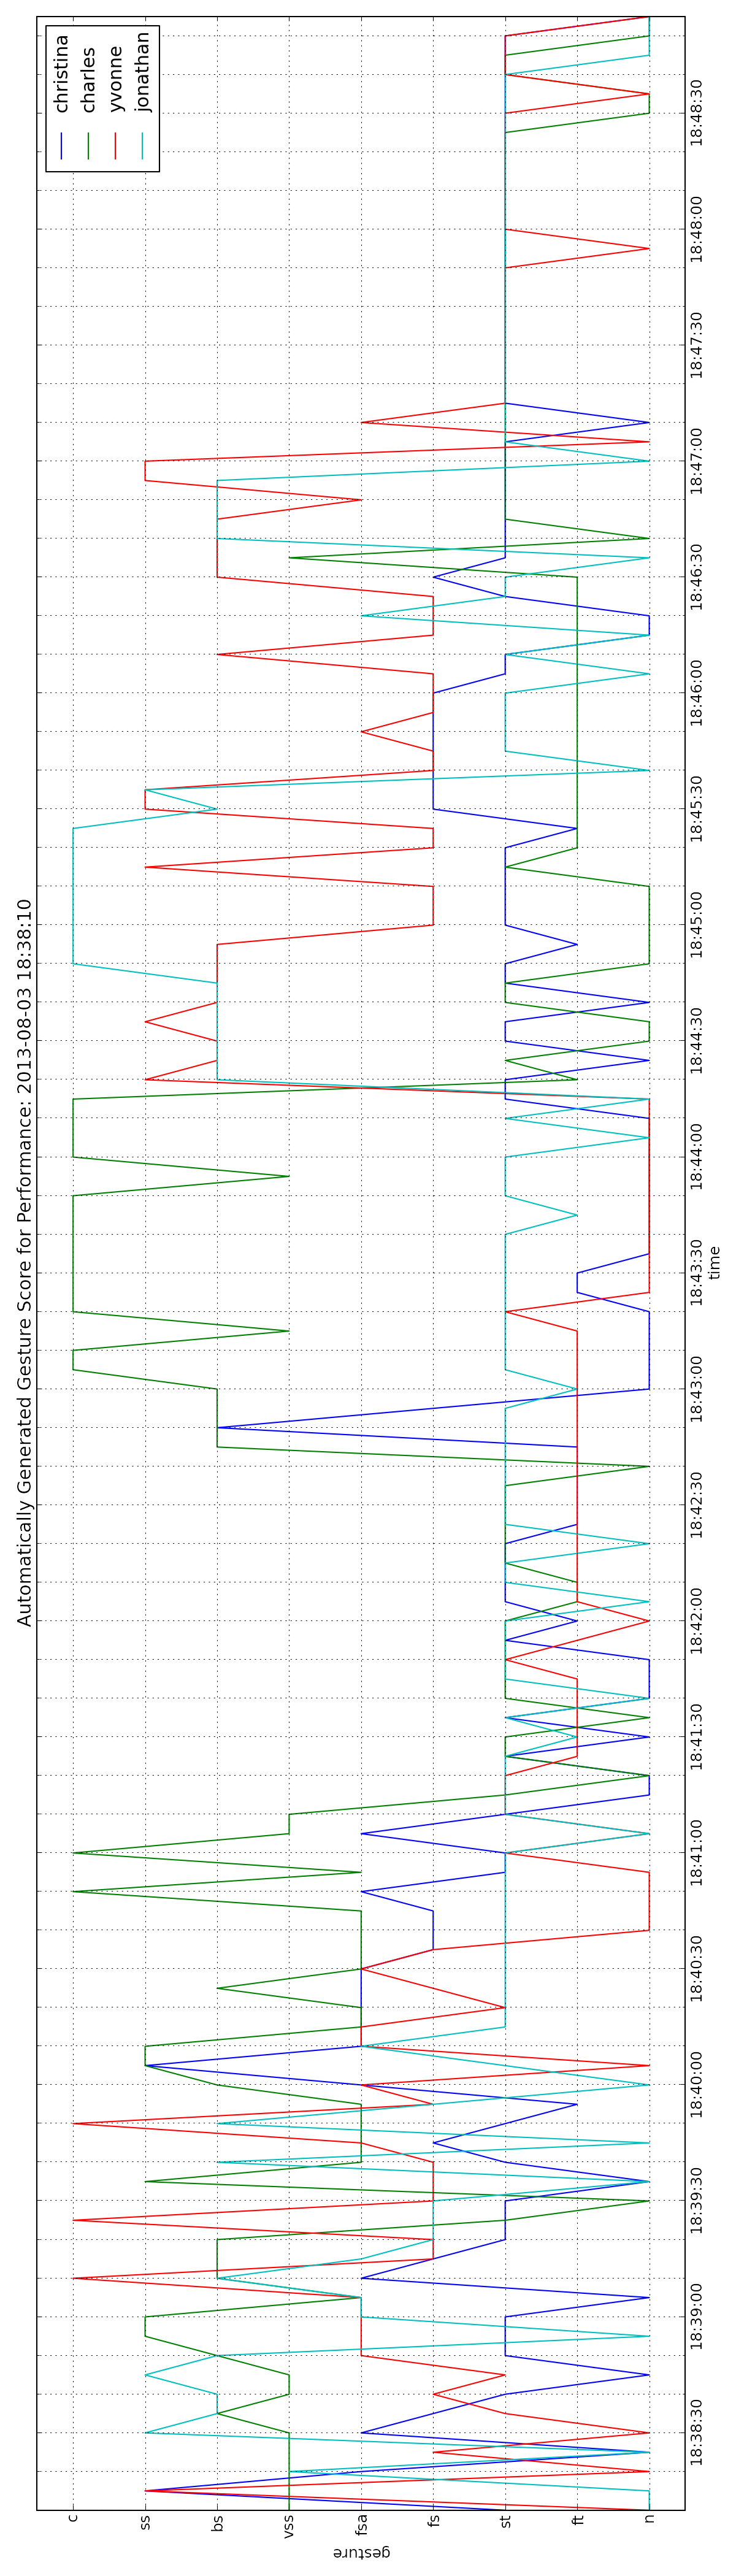
\includegraphics[height=0.9\textheight]{figures/score20130803vert}
\caption{An automatically generated ``gesture score'' for the
  \emph{MetaLonsdale} performance on 3-8-2013. }
\label{gesturescore}
\end{figure}


% \subsection{Tracking Gestures as a Score}
% \label{subsec:gesture-scores}


\subsection{Identifying Special Events}
\label{subsec:special-events}

Some aspects of musical structure in touch-screen improvisations are
visually apparent in graphical gesture scores, but it is also possible
to automatically discriminate between different styles of touch-screen
performance and identify transitions between multiple sections. To
analyse such features, the performance of all performers in an
ensemble must be considered at once, and our time series of gestural
classifications are an ideal format for exploring these ensemble
interactions. The method used in our Metatone Classifier software is
that of transition matrix analysis~\cite{Swift:2014tya}, where
performers' changes between gestures are summarised in matrices
allowing simultaneous analysis of the whole ensemble over varying
windows of time, or over a whole performance. In Metatone Classifier,
transition matrices of gesture groups are calculated over 15-second windows, each second
during a performance, a value determined through a process of trial
and error. Once a transition matrix has been produced, several
measures can be applied to them with little computational cost, an
important factor in a real-time application. Out of several
experimental tests on transition matrices, our \emph{flux} measure~\cite{Martin:2015jk} has
proven to be extremely promising. Flux is a measure of the rate of
gestural change calculated by dividing the number of transitions from
one gesture to another by the self-transitions where a gesture is
followed by itself. The value of flux is maximised at 1 when no
gesture follows itself, and is minimised at 0 when each member of the
ensemble stays on the same gesture for the whole window of
calculation. When applied on a window of calculation that slides over
a whole performance, peaks in flux tend to match moments where the
ensemble shifts to a new section. In Metatone Classifier we have
implemented a strategy that tracks sudden increases in flux to
identify these new ideas.

When our software identifies one of these events during a performance,
an OSC message is sent to each of the connected iPad apps. As part of
our research program, we have experimented with a number of responses
in the app interfaces for these messages~\cite{Martin:2015jk}. The
apps might display a series of new notes to reward the performers or
progress through a composition of sound scapes to encourage further
exploration. One controversial app was designed to disrupt the
performers while a new-idea message had \emph{not} been triggered to
forcefully encourage them to try something new.

As with all of our app-server interactions, new-idea messages are
logged in our performance protocols and have been useful in later
analysis of improvised performances. These messages are shown in
Figure \ref{gesturescore} as vertical red lines. Since calculations
over several seconds may identify the same increase in flux, new-idea
messages are often grouped together closely although our apps are
designed to ignore messages that arrive more frequently than once
every ten seconds. 

\subsection{Visualisations}
\label{subsec:visualisations}

To understand the structure of the improvised performances we wanted a
visual representation of the performers' touch gestures to watch
alongside the audio and video recordings of each performance. A
Processing sketch was produced that read the captured log files and
rendered an animation of all four players' touches in the space of one
iPad screen with different players distinguished by colour. The sketch
also draws a date and time stamp on each frame as well as text
notifications of switch and button messages.

The resulting animations presents an entirely new view of the
performance which was not visible to the performers or audience on the
day. As all the touch movements are layered in one performance area it
is immediately clear when performers mimic each other, form sections,
or experiment with a new musical idea. From the researcher's point of
view, the animation also gives a ``performer's perspective'' on touch
interaction, allowing us to connect patterns of touches with musical
gestures that the performers discuss after rehearsals.



\section{Conclusions}

By logging touch-interactions in Ensemble Metatone's performances on
iPads we recorded aspects of the musical work that are not accessible
in traditional archives of free-improvised music. The logs also allow
further insight into the gestural nature of performance on
touch-screens. In particular, animations of the performers' touches
aided the development of a vocabulary of gestures. Graphical ``gesture
scores'' following this vocabulary were generated from the logs
automatically using a Machine-Learning algorithm.

These alternative representations have allowed a more comprehensive
archive of performances and one that affords more insight into the
performers' gestural and musical intent and ensemble interactions as
well as their sonic output. As more performances are logged, it is
hoped that these representations will allow us to track the group's
musical developments or different approaches taken with future touch
instruments. The representations could also be used in performance as
visual accompaniments for the audience or displayed to the players as
real-time feedback.

\bibliographystyle{spphys}
\bibliography{2013ComputerMusic}
\end{document}

% %
% \section*{Appendix}
% \addcontentsline{toc}{section}{Appendix}
% %
% %
% When placed at the end of a chapter or contribution (as opposed to
% at the end of the book), the numbering of tables, figures, and
% equations in the appendix section continues on from that in the main
% text. Hence please \textit{do not} use the \verb|appendix| command
% when writing an appendix at the end of your chapter or contribution.
% If there is only one the appendix is designated ``Appendix'', or
% ``Appendix 1'', or ``Appendix 2'', etc. if there is more than one.
